\Chapter{Die ASCII-Unit}

\label{ch:asciiunit}
Die ASCII-Unit stellt die grafische Schnittstelle zwischen Prozessor und Benutzer dar, und fungiert somit als Hauptinterface, die implementierte Funktionalit\"at auf dem Monitor darzustellen.

\begin{figure}[!htbp]
	\centering
	\label{fig:exampletext}
	\includegraphics[width=0.7\textwidth]{asciiunitexample.png}
	\caption[Beispiel f\"ur die Textausgabe]{Beispiel f\"ur die Textausgabe: jedes darstellbare Zeichen wird abgebildet}
\end{figure}

\Section{\"Uberblick}

Die ASCII-Unit gibt auf dem Monitor, der \"uber die VGA-Schnittstelle des Entwicklungsboards angeschlossen wird, mittels Memory-Mapping den Inhalt des CHARRAM-Blocks in Form von ASCII-Zeichen wieder. Dazu wird jeweils eine Speicheradresse auf eine bestimmte Position auf dem Monitor wie folgt abgebildet: Das Offset 0 repr\"astentiert das erste Zeichen (linkes oberes Eck), wobei mit jedem Schritt nach rechts das zugrundeliegende Offset inkrementell anw\"achst. Auf den letzten Buchstaben in einer Zeile folgt direkt der erste Buchstabe der darunter liegenden. So ergibt sich - analog zu einem zweidimensionalen Array - ein Zeilenumbruch nicht durch ein entsprechendes Steuerzeichen, sondern ist durch den Offset automatisch implizit gegeben. Es ergeben sich auf diese Weise 32 Zeilen mit je 16 Buchstaben, sodass insgesamt 2048 verschiedene ASCII-Character dargestellt werden k\"onnen. Die Basisadresse f\"ur den beschriebenen Speicherbereich stellt direkt die Basisadresse des CHARRAM-Blocks der MMU(\ref{ch:mmu}) dar.

Um ein Zeichen anhand seiner ASCII-Nummer darzustellen, wurde eine CHARMAP implementiert, die zu jedem der 256 ASCII Zeichen einen 64-Bit-Vektor bereitstellt hat. Dieser ist wiederum schlicht eine 8*8 Bitmap der Farbtiefe 1 BPP, sodass ein Character theoretisch den gesamten f\"ur ihn reservierten Bildschirmbereich erfassen kann. Allerdings  werden von diesen 64 Bit jeweils immer nur nur 6*6 tats\"achlich benutzt, woraus ein Zeilenabstand von 2 Pixeln resultiert. Diese im Bezug auf Ausnutzung des vorhandene Speicherplatzes zwar nicht die optimale Umsetzung, erm\"oglichte allerdings eine einfache Implementierung; Positionelle Berechnungen, die unter anderen auf arithmetische Operationen wie Multiplikation und Division (welche aber nicht vom Rechenwerk \"ubernommen werden k\"onnen) zur\"uckgreifen, sind auf ganzzahligen Potenzen von 2 erheblich einfacher und weniger zeitintensiv zu realisieren.

\begin{figure}[H]
	\centering
		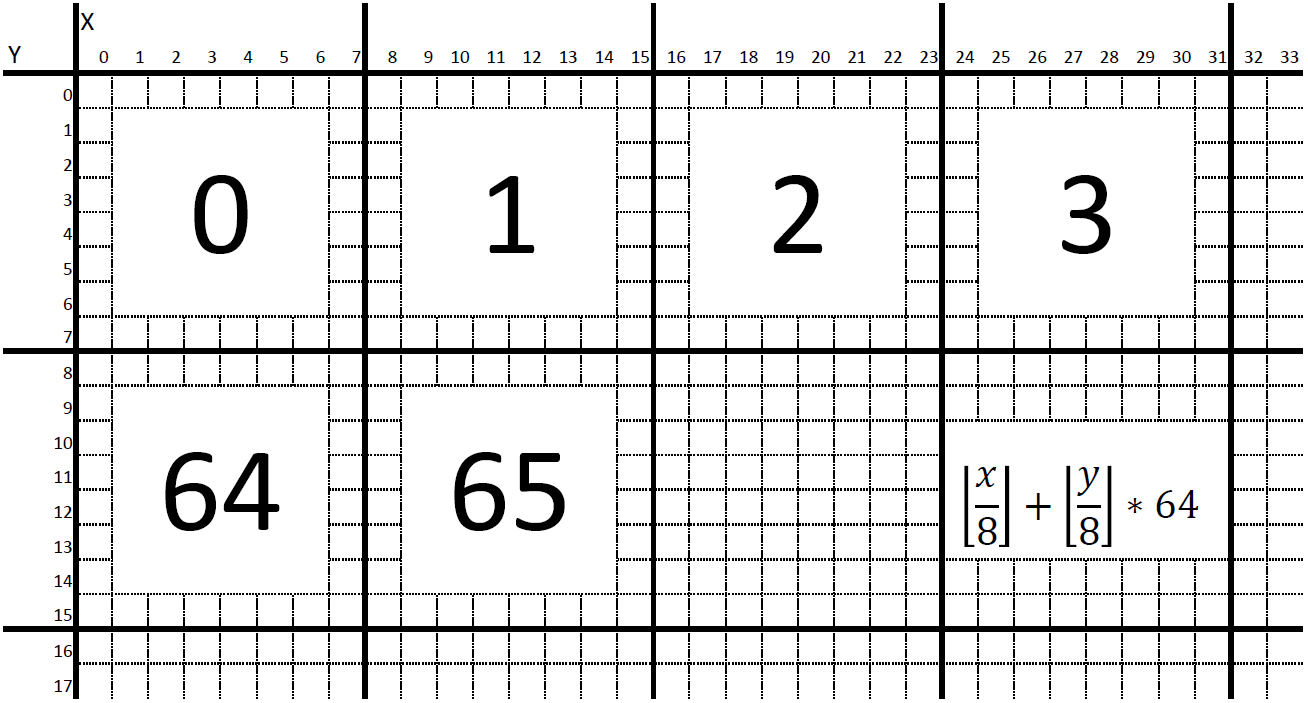
\includegraphics[width=1.0\textwidth]{Bildschirm.png}
	\caption[Veranschaulichung der Adressberechnung der ASCII-Unit]{Veranschaulichung der Adressberechnung anhand des Pixelfelds des Monitors: Links oben wird von 0 ab nach rechts inkrementell iteriert. Die Adresse des Zeichenfeldes, das auf die Position (x,y) abbildet, errechnet sich wie folgt: $\lfloor \frac{x}{8} \rfloor + \lfloor \frac{y}{8} \rfloor * 64$. Aus dem 64-Bit-Vektor wird man das Bit f\"ur den aktuelle Pixel bestimmt: $(x\:  mod\:  8) + (y\:  mod\:  8) * 8$}
\end{figure}

Da eine Darstellung von Kleinbuchstaben innerhalb einer 6*6 Bitmap nur wenig Unterschied zur analogen Implementierung von Gro\ss{}buchstaben aufweist und eine Unterscheidung deshalb ohnehin nur schwerlich m\"oglich w\"are, greifen auch diese auf die Bitmaps der entsprechenden Gro\ss{}buchstaben zur\"uck. Aus der oben beschriebenen Implementierung geht direkt hervor, dass Steuerzeichen wie Tabulatoren oder Zeilenumbr\"uche keinerlei Effekt haben und deswegen auf leere Zeichen gemappt sind. Dies hat allerdings zur Folge, dass die Textformatierung durch entsprechende Software \"ubernommen werden muss.

Die ASCII-Unit wird, um die VGA-Schnittstelle ansprechen zu k\"onnen, mit 25 MHz getaktet. Dabei sendet die VGA-Unit mit jeder Taktflanke einen weiteren Pixel an das angeschlossene Ger\"at, wobei die Farbinformation sich dabei aufgrund der Farbtiefe von 1 BPP auf Schwarz/Wei\ss{} beschr\"ankt. Die Berechnung dieser Farbinformation erfolgt innerhalb der ASCII-Unit stufenweise und f\"ur jeden Pixel pro Taktflanke. 

\Section{Interface}
Neben dem bereits erw\"ahnten Takteingang gibt es jeweils einen Eingang f\"ur die x- und y-Koordinate des aktuellen Pixels (bzw. Position des Fadenstrahls) aus der VGA-Unit, welche mit jedem Takt aktualisiert werden und ein Ausgangssignal an die VGA-Einheit, welches angibt, ob das aktuelle Pixel gesetzt werden soll oder nicht.\\ Au{\ss}erdem gibt es zur Kommunikation mit dem CHARRAM in der MMU einen Ausgang, welcher die Adresse des Zeichenplatzes des aktuell zu berechnenden Pixels angibt sowie einen Eingang, der im darauffolgenden Takt die ASCII-Nummer des zugeh\"origen Zeichens erh\"alt.\\
Zur CHARMAP, die als ROM fungiert, wird der Takt durchgeleitet und ebenso die aus dem CHARRAM kommende ASCII-Nummer des aktuellen Zeichens, die hierbei als Adresse auftritt. Aus der CHARMAP kommt im darauffolgendem Takt der oben erw\"ahnte 64-Bit-Vektor der das jeweilige Zeichen repr\"asentiert.

\begin{figure}[H]
	\centering
	\label{fig:interface}
		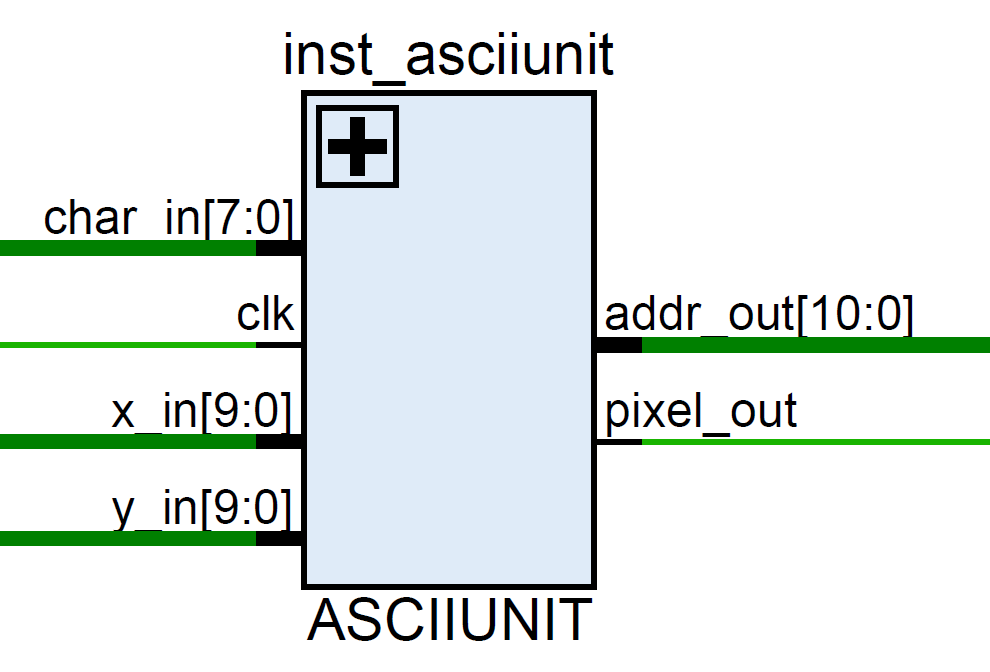
\includegraphics[width=0.3\textwidth]{Asciiunit.png}
	\caption[Interface der ASCII-Unit]{Das Interface der ASCII-Unit}
\end{figure}

\Section{Funktionsweise}

Da die stufenweise Berechnung der zu einer Position geh\"orenden Farbinformation mehr als einen Takt ben\"otigt, errechnet die ASCII-Unit diese bereits zwei Takte im Voraus: Dazu wird zun\"achst die Position des n\"achsten zu zeichnenden Bildschirmpixels eingelesen und die X-Koordinate um den Wert zwei inkrementiert. Dann beginnt die eigentliche Berechnung, die genau dann rechtzeitig beendet sein wird, wenn die VGA-Unit die entsprechende Bildschirmposition erreicht.

Im darauf folgenden Takt wird aus der Positionsinformation der zugrundeliegende Offset innerhalb des CHARRAM-Blocks errechnet und an die MMU weitergeleitet. Dabei wird nicht das Zugriffsprotokoll, \"uber welches das Leitwerk mit der MMU kommuniziert, verwendet; stattdessen erfolgt der Datenaustausch zwischen dem CHARRAM-Controller und der ASCII-Unit direkt durch weitergeleitete Signale innerhalb der MMU. Dies begr\"undet sich darin, dass die ASCII-Unit konstant mit Daten versorgt werden muss und ein regul\"arer Speicherzugriff dieser Anforderung nicht gen\"ugt. Der CHARRAM-Controller kann diesen gegebenenfalls zweiten lesenden Speicherzugriff insofern verarbeiten, dass der RAM-Block als Dual-Port-Blockram realisiert wurde. Ebenso spielt die asynchrone Taktfrequenz der MMU hierbei keinerlei entscheidende Rolle, da schlimmstenfalls derselbe Lesezugriff mehr als einen Takt anliegt, was aber die Valididt\"at der Daten keineswegs beeinflusst. Einzig gleichzeitig schreibende und lesende Zugriffe auf ein und dieselbe Speicherzelle verursachen kurzweilige Probleme, da die ausgegebenen Farbinformationen in diesem Fall nicht den gespeicherten Daten entsprechen. Allerdings h\"alt dieser fehlerhafte Zustand nur bis zum erneuten Zeichnen der entsprechenden Speicherposition an, sodass die fehlerhafte Darstellung mit blo\ss{}em Auge nicht zu erkennen ist.

Um anhand des ASCII-Codes einer Speicheradresse die der Position entsprechende Farbinformation innerhalb des derzeitigen Zeichens zu erhalten, wird die eingangs erw\"ahnte CHARMAP ausgelesen. Dazu wird die ben\"otigte Bitmap angefragt und dann entsprechend der Bildschirmposition ausgewertet. 

Zuletzt wird die resultierende Farbinformation dann an die VGA-Unit, welche nun erst die errechnete Bildschirmposition erreicht hat, weitergeleitet, wobei im Hintergrund bereits, \"ahnlich einer Pipeline, die Verarbeitung der folgenden Pixel im Gange ist.

\begin{figure}[H]
	\centering
	\label{fig:overview}
		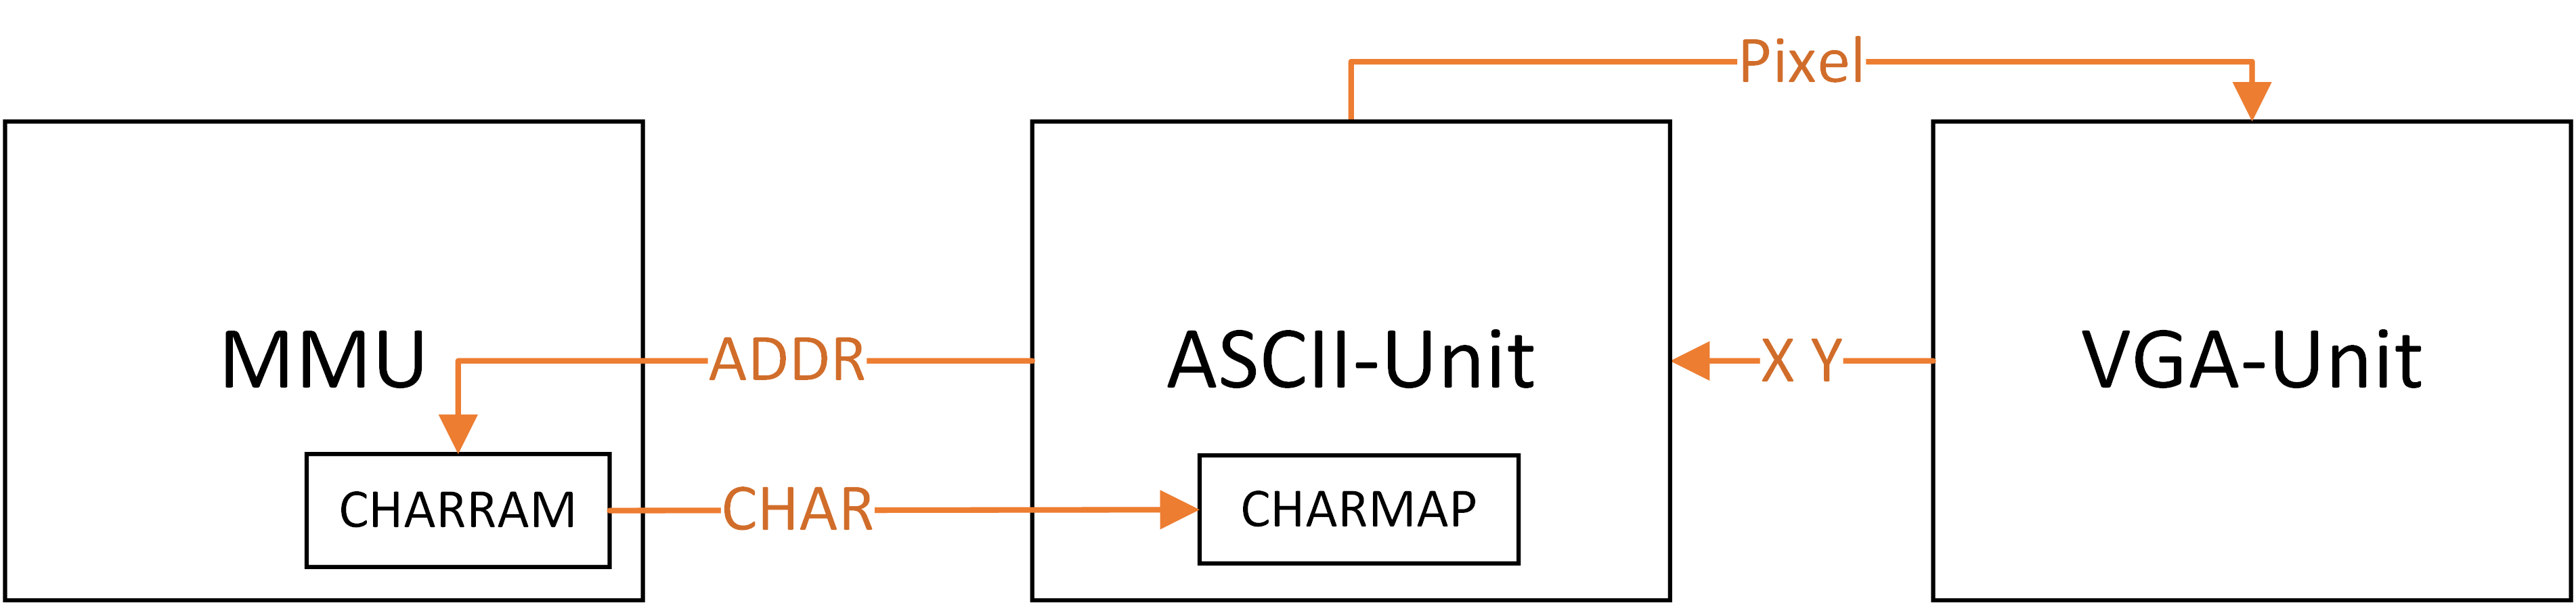
\includegraphics[width=1.0\textwidth]{ASCII.png}
	\caption[\"Ubersicht \"uber die ASCII-Unit]{\"Ubersicht: Beginn bei x- bzw. y-Koordinate; Verrechnung dieser zur Adresse f\"ur CHARRAM; dann Durchleiten in CHARMAP; anschlie\ss{}end Berechnung des Pixels; letztendlich Zur\"ucksenden an VGA-Unit}
\end{figure}

\newpage


